% \documentclass[tikz,border=3.14mm]{standalone}
% \usetikzlibrary{decorations.pathmorphing}
% \begin{document}
% % \begin{tikzpicture}
% %     \clip (-1,-1) rectangle (31,12);
% %     \foreach \X in {1,2,...,10}
% %     {\foreach \Y in {1,2,...,10}
% %     {\node[circle,text=white,font=\sffamily\bfseries\large,inner color=blue,outer color=blue] at (\X,\Y) {};}};
% %     \foreach \X in {11,12,...,20}
% %     {\foreach \Y in {1,2,...,10}
% %     {\node[circle,text=white,font=\sffamily\bfseries\large,inner color=red, outer color=red] at (\X,\Y) {};}};
% %     \foreach \X in {21,22,...,30}
% %     {\foreach \Y in {1,2,...,10}
% %     {\node[circle,text=white,font=\sffamily\bfseries\large,inner color=blue,outer color=blue] at (\X,\Y) {};}};
% %     \node[] at (5,11)  {\huge Altermagnet};
% %     \node[] at (15,11) {\huge Superconductor};
% %     \node[] at (25,11) {\huge Altermagnet};
% %     \end{tikzpicture}
% %\begin{tikzpicture}
%     % \clip (-1,-1) rectangle (31,22);
%     % \foreach \X in {1,2,...,10}
%     % {\foreach \Y in {-\X,..., \X}
%     % {\node[circle,text=white,font=\sffamily\bfseries\large,inner color=blue,outer color=blue] at (\X,20 -\X - \Y) {};}};
% %\end{tikzpicture}
% \begin{tikzpicture}[scale=0.5,rotate=-45]
%   \draw[thick,-] (-5,0) -- (5,0);
%   \draw[thick,-] (0,-5) -- (0,5);
%   \foreach \x in {-4,...,4}
%     \foreach \y in {-4,...,4}
%       \filldraw [blue] (\x,\y) circle (0.2);
% \end{tikzpicture}
% \end{document}
% \end{document}
\documentclass{standalone}
\usepackage{tikz}
\usepackage[utf8]{inputenc}
\usepackage[T1]{fontenc} % To write accents/acute like \'i
\usepackage{newtxtext}
\usepackage[upint]{newtxmath}
\usepackage{microtype}
\usepackage{textcomp}
\usepackage{eucal}
\usepackage{bm}
\usepackage{siunitx}
\usepackage{comment}
\usepackage{lipsum}
\begin{document}

% \begin{tikzpicture}[scale=0.5, rotate=0]
%     % define lattice parameters
%     \def\a{1} 
%     % \def\halfa{0.5*\a}
%     \filldraw[blue] ({3.},{12}) circle (0.4);
%     \node at (6.5, 12) {\Large Altermagnet};

%     \filldraw[red] ({12.},{12}) circle (0.4);
%     \node at (16, 12) {\Large Superconductor};

%     \foreach \i in {1,...,20} {
%       \foreach \j in {1,...,10} {
%         \ifnum\i>10 % check if j is greater than 2
%             \filldraw[red] ({\i*\a},{\a*\j}) circle (0.2);
%         \else
%             \filldraw[blue] ({\i*\a},{\a*\j}) circle (0.2);
%             \fi
%       }
%     }
%     % To include a second AM
%     % \foreach \i in {21,...,30} {
%     %   \foreach \j in {1,...,10} {
%     %     \pgfmathtruncatemacro\parity{mod(\i,2)}
%     %     \ifnum\parity=1
%     %         \filldraw[blue] ({\i*\a/2},{\a*\j}) circle (0.2);
%     %     \else
%     %         \filldraw[blue] ({\i*\a/2},{\a*\j-0.5*\a}) circle (0.2);
%     %     \fi
%     %   }
%     % }
%   \end{tikzpicture}
% % ------------------------------------------------------


% \begin{tikzpicture}[scale=0.5]
%      % Draw coordinate axes
%   \draw[->] (-0.1, 0) -- (2, 0) node[right] {$x$};
%   \draw[->] (0, -0.1) -- (0, 2) node[above] {$y$};
% \end{tikzpicture}

%   \begin{tikzpicture}[scale=0.5, rotate=135]
%     % define lattice parameters
%     \def\a{sqrt(2)} 
%     \def\halfa{0.5*\a}
% %      % Draw coordinate axes
%   % \draw[->] (-0.1, 0) -- (2, 0) node[right] {$x$};
%   % \draw[->] (0, -0.1) -- (0, 2) node[above] {$y$};

%     % draw lattice points
%     \foreach \i in {1,...,20} {
%       \foreach \j in {1,...,5} {
%         \pgfmathtruncatemacro\parity{mod(\i,2)}
%         \ifnum\parity=1
%             \ifnum\i>10 % check if j is greater than 2
%                 \filldraw[blue] ({\i*\a/2},{\a*\j}) circle (0.2);
%             \else
%                 \filldraw[red] ({\i*\a/2},{\a*\j}) circle (0.2);
%                 \fi
%         \else
%           \ifnum\i>10 % check if j is greater than 2
%             \filldraw[blue] ({\i*\a/2},{\a*\j-0.5*\a}) circle (0.2);
%           \else
%             \filldraw[red] ({\i*\a/2},{\a*\j-0.5*\a}) circle (0.2);
%           \fi
%         \fi
%       }
%     }
%     % \foreach \i in {21,...,30} {
%     %   \foreach \j in {1,...,10} {
%     %     \pgfmathtruncatemacro\parity{mod(\i,2)}
%     %     \ifnum\parity=1
%     %         \filldraw[blue] ({\i*\a/2},{\a*\j}) circle (0.2);
%     %     \else
%     %         \filldraw[blue] ({\i*\a/2},{\a*\j-0.5*\a}) circle (0.2);
%     %     \fi
%     %   }
%     % }
%   \end{tikzpicture}
%------------------------------------------------


% -- Make the d-wave structure 1 --
% \begin{tikzpicture}
%          % Draw coordinate axes
%     \draw[->] (-4.1, 0+ 6.5) -- (0, 6.5) node[right] {$x$};
%     \draw[->] (-4, -0.1+6.5) -- (-4, 4 + 6.5) node[above] {$y$};
%     % Draw the d-wave
%     \def\h{1.5}
%     \def\w{0.8}
%     \draw (-4, 5) ellipse (\w cm and \h cm);  % Draw labels
%     \draw (-4, 8) ellipse (\w cm and \h cm); 
%     \draw (-2.5, 6.5) ellipse (\h cm and \w cm);
%     \draw (-5.5, 6.5) ellipse (\h cm and \w cm);

%     \node[draw=red, fill=red, line width=0.5pt, minimum width=0.75cm, minimum height=0.075cm] (horizontal) at  (-5.5, 6.5) {};
%     \node[draw=red, fill=red, line width=0.5pt, minimum width=0.75cm, minimum height=0.075cm] (horizontal) at  (-2.5, 6.5) {};

%     \node[draw=blue, fill=blue, line width=0.5pt, minimum width=0.75cm, minimum height=0.075cm] (horizontal) at (-4, 8) {};
%     \node[draw=blue, fill=blue, line width=0.5pt, minimum width=0.075cm, minimum height=0.75cm] (vertical) at (-4, 8) {};
%     (-1.5, 6.5) 
    

%     \node[draw=blue, fill=blue, line width=1pt, minimum width=0.75cm, minimum height=0.075cm] (horizontal) at  (-4, 5) {};
%     \node[draw=blue, fill=blue, line width=0.5pt, minimum width=0.075cm, minimum height=0.75cm] (vertical) at (-4, 5) {};

%     % Draw spin
%     \draw [->, line width = 3pt] (-2, 0+ 7.5) -- (-2, 1.5+ 7.5) node[right] {Spin up};
% \end{tikzpicture}
% ---------------------------------------------
% -- Make the d-wave structue 2 --
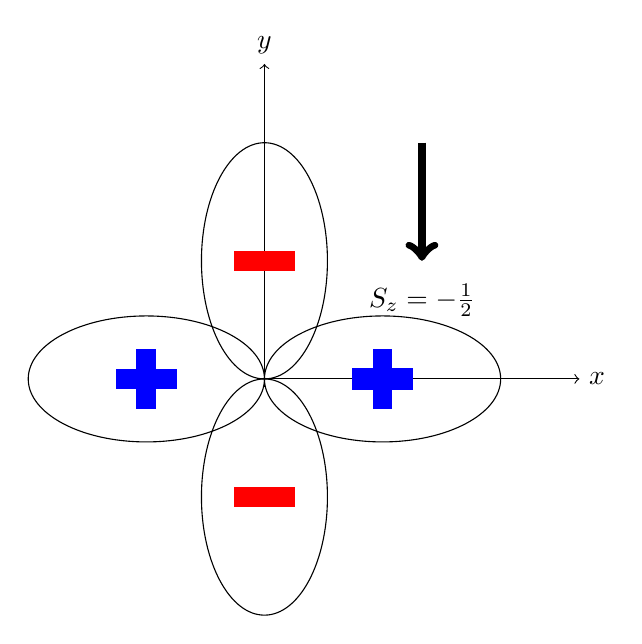
\begin{tikzpicture}
         % Draw coordinate axes
    \draw[->] (-4.1, 0+ 6.5) -- (0, 6.5) node[right] {$x$};
    \draw[->] (-4, -0.1+6.5) -- (-4, 4 + 6.5) node[above] {$y$};
    % Draw the d-wave
    \def\h{1.5}
    \def\w{0.8}
    \draw (-4, 5) ellipse (\w cm and \h cm);  % Draw labels
    \draw (-4, 8) ellipse (\w cm and \h cm); 
    \draw (-2.5, 6.5) ellipse (\h cm and \w cm);
    \draw (-5.5, 6.5) ellipse (\h cm and \w cm);

    \node[draw=red, fill=red, line width=0.5pt, minimum width=0.75cm, minimum height=0.075cm] (horizontal) at  (-4, 8) {};
    
    \node[draw=red, fill=red, line width=0.5pt, minimum width=0.75cm, minimum height=0.075cm] (horizontal) at  (-4, 5) {};

    \node[draw=blue, fill=blue, line width=0.5pt, minimum width=0.75cm, minimum height=0.075cm] (horizontal) at(-5.5, 6.5)  {};
    \node[draw=blue, fill=blue, line width=0.5pt, minimum width=0.075cm, minimum height=0.75cm] (vertical) at (-5.5, 6.5) {};
    (-1.5, 6.5) 
    

    \node[draw=blue, fill=blue, line width=1pt, minimum width=0.75cm, minimum height=0.075cm] (horizontal) at  (-2.5, 6.5) {};
    \node[draw=blue, fill=blue, line width=0.5pt, minimum width=0.075cm, minimum height=0.75cm] (vertical) at (-2.5, 6.5) {};

    % Draw spin
    \draw [->, line width = 3pt] (-2, 9.5 ) -- (-2, 8.) node[right] {};

    \node[]  at (-2, 7.5) {$S_z=- \frac{1}{2}$};
\end{tikzpicture}
\end{document}
